\section{Domain Adaptation}
\label{sec:Chapter3} \index{Chapter3}

В современном мире машинного обучения и искусственного интеллекта способность моделей адаптироваться к новым условиям и данным стала одной из ключевых задач. Традиционные методы обучения моделей предполагают, что данные, используемые для обучения и тестирования, имеют схожие характеристики и распределения. Однако в реальных приложениях часто возникает необходимость применять модели на данных, которые существенно отличаются от тех, на которых они были изначально обучены. Это приводит к снижению точности и эффективности моделей, что ставит под угрозу их практическое применение.

Для решения данной проблемы была разработана задача доменной адаптации, целью которой является создание методов для акклиматизации модели к целевым данным, отличающимся от исходных. В рамках этой задачи были разработаны подходы и техники, направленные на уменьшение расхождений между исходным и целевым доменами, что позволяет сохранять точность и производительность моделей в новых условиях. Эти методы способствуют переносу знаний, накопленных в исходном домене, на целевой, что относит данную задачу к области методов transfer learning.

\subsection{Перенос знаний}

ЗДЕСЬ ТОЧНО НАДО БУДЕТ ИСПОЛЬЗОВАТЬ КАРТИНКУ ДЛЯ ОПИСАНИЯ ЧТО ТАКОЕ ПЕРЕНОС ОБУЧЕНИЯ

\begin{figure}[h]
	\centering
	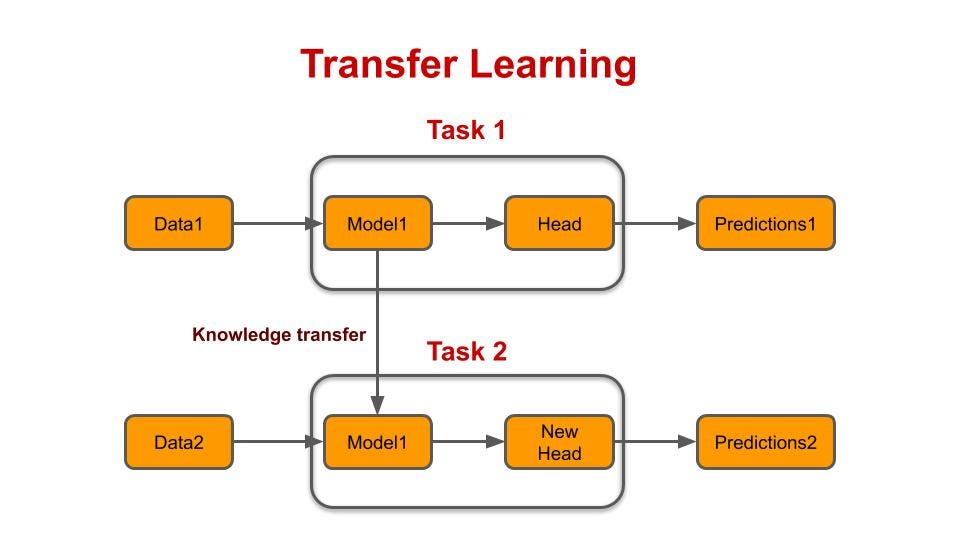
\includegraphics[width=.9\textwidth]{./images/TL_medium.jpg}
	\caption{Основная идея переноса знаний\\ИСТОЧНИК}
	\label{fig:tl}
\end{figure}

СЛЕДУЮЩИЕ АБЗАЦЫ ДО МЕТКИ НЕОБХОДИМО ПРОВЕРИТЬ И ВОЗМОЖНО ПЕРЕНЕСТИ ВО ВВЕДЕНИЕ

Обучение модели и разработка алгоритма её работы представляют собой чрезвычайно сложный и трудоемкий процесс. Этот процесс требует значительных ресурсов, как со стороны специалистов, так и в плане вычислительной мощности. Сначала необходимо собрать и подготовить данные, затем обучить модель, настроить её параметры и протестировать на различных наборах данных, чтобы убедиться в её точности и надёжности. Это часто занимает много времени и требует значительных финансовых вложений. 

Столкнувшись с этими трудностями, исследователи начали искать способы повысить эффективность и упростить процесс обучения моделей. Они пришли к идее использования знаний, полученных при решении одной задачи, для решения другой, сходной задачи. Такой подход получил название \textit{переноса обучения (англю. transfer learning)}. Он позволяет существенно сократить время и ресурсы, необходимые для разработки новых моделей, путём повторного использования уже существующих знаний и наработок.

%%ВЫГЛЯДИТ КАК АБЗАЦ ДЛЯ ВВЕДЕНИЯ :) Или нет :)

Суть переноса обучения заключается в том, что модель, предварительно обученная на одном наборе данных, может быть адаптирована для работы на другом наборе данных, даже если они различаются по своему содержанию или структуре. Например, модель, обученная на огромном корпусе текстов, может быть успешно применена для анализа тональности текстов или для распознавания именованных сущностей в другом наборе данных. Точно так же, модели, обученные на больших наборах изображений, могут быть использованы для решения задач распознавания объектов или классификации изображений в других доменах. (см \autoref{fig:tl})

Поэтому исследователи задались вопросом применении знаний, полученных в результате решения одной задачи, для решения другой задачи. Такой процесс получил название \textit{переноса обучения (англю. transfer learning)}.  

МЕТКА ДО КОТОРОЙ НАДО ПРОВЕРЯТЬ АБЗАЦЫ

\subsection{Доменная адаптация}

В даннойчасти необходимо рассказать как из второго появилось первое.

\subsubsection{Классификация методов доменной адаптации}

Есть ли деление в доменной адаптации. Какое, какие бывают виды. Провести обзор.

ЗДЕСЬ ТОЧНО НАДО БУДЕТ ИСПОЛЬЗОВАТЬ КАРТИНКУ КАК В ПРЕЗЕНТАЦИИ ДЛЯ КЛАССИФИКАЦИИ МЕТОДОВ ДА

\newpage